\documentclass[12pt, a4, twoside]{article}
\usepackage[utf8]{inputenc}
\usepackage{graphicx}
\usepackage{algorithm}
\usepackage{algpseudocode}
\usepackage{amsmath}
\usepackage{amsfonts}
\usepackage{hyperref}
\usepackage{mathtools}
\usepackage{amssymb}

\DeclarePairedDelimiter\ceil{\lceil}{\rceil}
\DeclarePairedDelimiter\floor{\lfloor}{\rfloor}

\hypersetup{
    colorlinks=true,
    linkcolor=blue,
    filecolor=magenta,
    urlcolor=cyan,
}

\newtheorem{theorem}{Theorem}[section]
\newtheorem{definition}{Definition}[section]
\newtheorem{notation}{Notation}[section]
\newtheorem{remark}{Remark}[section]
\newtheorem{corollary}{Corollary}[theorem]
\newtheorem{lemma}[theorem]{Lemma}
\newtheorem{problem}[theorem]{Problem}

\usepackage[backend=bibtex]{biblatex}
\addbibresource{integral-equations.bib}

\title{Integral Equation Methods for Problems In Scientific Computing}
\author{Srinath Kailasa \thanks{srinath.kailasa.18@ucl.ac.uk} \\ \small University College London}

\date{\today}

\begin{document}

\maketitle

\section*{Abstract}

Integral equations are an invaluable tool in scientific computing for formulating and solving scattering problems. This is because they allow for a reduction in problem dimension, by discretising and solving a problem over the surface of the scatterer to find a solution over the whole domain. The focus of this document is to summarise the main aspects of integral equations as they relate to scattering problems. The notes are written for my own selfish clarity rather than neatness, or succinctness, of mathematical arguments. I hope they are useful to read as they were to write \footnote{These notes were written up during my visit to the Flatiron Institute in New York City in the Summer of 2022. A wonderful experience for which I am extremely grateful. The visit gave me both the impetus and the time to study some truly interesting and beautiful concepts.}.

\newpage

\tableofcontents


\section{Mathematical Background}\label{sec:mathematical_background}

Some facts from functional and real analysis are unavoidable. Though I will try and keep them as wordy as possible. The main theory we rely on is that of Fredholm and Riesz. In terms of function spaces, we're going to assume that the only domains I will ever see are nice and smooth, with no cracks or edges, and will therefore ignore much of the function-space formalism for the time being. I \textit{might} return to this later, if I really must. I have found some excellent lecture notes \cite{moiola2022} which give an overview of this type of formalism with application to boundary integral equations. I'm following along with the presentation in \cite{coltonkress2013,kress2012}, in addition to my own expository notes.


We're concerned with solving \textit{integral} equations of the form,

\begin{flalign}
    \label{eq:int_eqs}    
    \int_a^b K(x, y) \phi(y)dy &= f(x), \> \> x \in [a, b] \\
    \phi(x) - \int_a^b K(x, y)\phi(y)dy &= f(x), \> \> x \in [a, b]
\end{flalign}

In operator form,

\begin{flalign}
    A \phi &= f \\
    \phi - A\phi &= f
\end{flalign}

Known as integral equations of the \textit{first} and \textit{second} kind respectively. The theory of Riesz-Fredholm for compact operators provide us a way to provably obtain uniqueness and existence for these equations.

Definitions and theorems listed are the ones I forget the most, I'm typing them out in an effort to internalise them,

\begin{definition}
    \label{def:compactness}
    A subset $U$ of a normed space $X$ is compact if every open covering of $U$ contains a finite subcovering, that is, for every family $V_j$, $j \in J$, of open sets with the property \cite{kress2012},

    \begin{equation}
        U \subset \cup_{j\in J} V_j
    \end{equation}

    There exists a finite sub-family $V_{j(k)}$, $j(k) \in J$, $k = 1...n$, with,

    \begin{equation}
        U \subset \cup_{k=1}^n V_{j(k)}
    \end{equation}
    A subset $U$ is sequentially compact if every sequence of elements from $U$  contains a subsequence converging to an element in U.
\end{definition}

Compact sets are bounded, closed and complete.

\begin{definition}
    \label{def:rel_comp}
    A subset of a normed spaces is called relatively compact if its closure is compact.
\end{definition}

\begin{theorem}[Arzela-Ascoli]
    \label{thm:arz-asc}
    A set $U \subset C(G)$, where $C(G)$ is the space of continuous functions defined on a compact set $G \subset \mathbb{R}^n$ with inf. norm,

    \begin{equation}
        \| \phi \|_\infty := \max_{x \in G} |\phi(x)| 
    \end{equation}

    is rel. compact iff it is bounded and equicontinuous. i.g. $\exists C$ s.t.,

    \begin{equation}
        |\phi(x)|  \leq C
    \end{equation}

    and $\forall x \in G$ and $\phi \in U$ and every $\epsilon > 0$ $\exists \delta > 0$ s.t.,

    \begin{equation}
        |\phi(x)-\phi(y)| < \epsilon
    \end{equation}

    for all $x,y \in G$ with $|x-y| < \delta$ and all $\phi \in U$
\end{theorem}

The above theorem of Arzela and Ascoli gives us a way to get the necessary and sufficient conditions for compactness on spaces of continuous functions. This will be useful later on when we're seeking compactness in our integral operators.

Compactness is a critical property for the operators that arise from integral equations. This is because, a compact operator $T: X \rightarrow Y$ maps bounded subsets of $X$ to relatively compact subsets of $Y$. Relatively compact means that the closure of a subset is compact. They are linear, and continuous

\subsection{Riesz Theory}

Riesz theory is concerned with second kind integral equations,

\begin{flalign}
    \phi - A \phi = f
\end{flalign}

Where $A: X \rightarrow X$ is a compact operator, that maps $X$ - a normed vector space to itself. A lot of the theorems below are stated without proof, the proofs are often long and technical to type out. And also not very interesting for my purposes. I'm interested only in seeing how the theorems are applied for solving integral equations.

Riesz's various theorems give us a way of determining whether solutions exist to equations of this form, and whether or not they are unique. We define $L := I-A$

\begin{theorem}[Riesz's First Theorem]
    The null space of $L$ is finite dimensional,
    $$N(L) := \{ \phi \in X: L \phi = 0 \}$$
\end{theorem}

Riesz gives us solvability in the case where $A$ is compact, demonstrating the importance of compactness.


\begin{theorem}[Riesz's Second Theorem]
    The range of $L$ is a closed linear subspace,
    $$ L(X) := \{ \phi \in X: \phi \in X \} $$
\end{theorem}

\begin{definition}
    \begin{flalign}
        L^n &= (I-A)^n = I - A_n \\
        \text{where, } A_n &= \sum_{k=1}^n (-1)^{k-1} {n \choose k} A^k
    \end{flalign}

    Is compact, where $N(L^n)$ is finite dimensional and $L^n(X)$ are closed subspaces.
\end{definition}

\begin{theorem}[Riesz's Third Theorem]
    There exists a uniquely determined non-negative integer $r$, called the Riesz number of an operator $A$, s.t.
    
    \begin{flalign}
        \{0\}  &= N(L^0) \subsetneqq N(L^1)  \subsetneqq ... \subsetneqq N(L^r)  = N(L^{r+1}) \\
        X &= L^0(X) \supsetneqq L^1(X) \supsetneqq ... \supsetneqq L^r(X) = L^{r+1}(X)
    \end{flalign}

    and,

    \begin{flalign}
        X = N(L^r) \oplus L^r(X)
    \end{flalign}

\end{theorem}

The two cases of interest are $r=0$ and $r>0$. This theorem is pretty abstract for me, and I'm struggling to see why it matters, except of course for the properties that are calculable from it.

\begin{theorem}
    Let $X$ be a normed vector space, $A: X\rightarrow X$ is a compact operator and $(I-A)$ is injective. Then the inverse operator $(I-A)^{-1}$ exists and is bounded.
\end{theorem}

The proof of the above is simple and is found on p 29 of \cite{kress2012}, as the operator $L$ is assumed to be injective $N(L) = 0$ by assumption, hence $r=0$. The main corollary of the theorem being a criterion for the solvability of second kind integral equations,

\begin{corollary}
    Let $X$ be a normed vector space, $A: X\rightarrow X$ is a compact operator. If the homogenous equation,

    \begin{flalign}
        \phi - A \phi = 0
    \end{flalign}
    only has the trivial solution $\phi=0$, then for all $f \in X$ the inhomogeneous equation,

    \begin{flalign}
        \phi - A \phi = f
    \end{flalign}
    has a unique solution $\phi \in X$, and this solution depends continuously on $X$.
\end{corollary}

Basically, if we can show our Riesz number to be 1, or equivalently that the null space of $L$ is just ${0}$, then Riesz theory guarantees us solvability of the inhomogeneous second kind linear integral equation. This all relies on the injectivity of $L$, if this is not the case we get the following theorem,

\begin{theorem}
    Let $X$ be a normed vector space, $A: X\rightarrow X$ is a compact operator, and assume $I-A$ is not injective. Then the null space $N(I-A)$ is finite dimensional and the range $(I-A)X \neq X$ is a proper closed subspace.
\end{theorem}

The proof of this is also simple, and comes from Riesz' theory. See p30 in \cite{kress2012}. Again, it's fairly abstract as a result, but it's basically saying that without injectivity, we loose the uniqueness of the inverse, and Riesz' theory has nothing more to say about the solvability of this system.

\begin{corollary}
    If the homogenous equation,

    \begin{flalign}
        \phi - A \phi = 0
    \end{flalign}
    has non-trivial trivial solutions then inhomogeneous equation,

    \begin{flalign}
        \phi - A \phi = f
    \end{flalign}

    is either unsolvable, or its general solution is of the form,

    \begin{flalign}
        \phi = \tilde{\phi} + \sum_{k=1}^m\alpha_k \phi_k
    \end{flalign}

    where $\phi_k$ are linearly independent solutions of the homogenous equation, and $\tilde{\phi}$ is a particular solution of the inhomogeneous equation.

\end{corollary}

This corollary is actually not useful, and this is where we need Fredholm theory, many real and useful formulations of boundary integral equations result in cases where the above corollary applies. We still want to solve these equations!

\subsection{Fredholm Theory}

Fredholm theory picks up where Riesz' theory tails off. We answer solvability for the systems in which $r>0$ by introducing some more mathematical machinery. Basically, compact operators are now considered in dual systems generated by non-degenerate bilinear - or more generally sesquilinear - forms. 

\begin{definition}
    Let $X, Y$ be linear spaces, A mapping $\langle \cdot , \cdot \rangle : X \times Y \rightarrow \mathbb{C}$ is called a bilinear form if,
    
    \begin{flalign}
        \langle \alpha_1 \phi_1 + \alpha_2 \phi_2,  \psi \rangle &= \alpha_1 \langle \phi_1, \psi \rangle + \alpha_2 \langle \phi_2, \psi \rangle \\
        \langle \phi, \beta_1\psi_1+\beta_2\psi_2 \rangle &= \beta_1 \langle \phi, \psi_1 \rangle + \beta_2 \langle \phi, \psi_2 \rangle
    \end{flalign}

    for all $\phi_1, \phi_2, \phi \in X$, $\psi_1, \psi_2, \psi \in Y$, and coefficients in $\mathbb{C}$. The bilinear form is non-degenerate if for every $\phi \in X, \phi \neq 0$ there exists $\psi \in Y$ s.t. $\langle \phi, \psi \rangle \neq 0$ and for every $\psi \in Y$ s.t.   $\langle \phi, \psi \rangle \neq 0$  there exists $\phi \in X$ s.t. $\langle \phi, \psi \rangle \neq 0$
\end{definition}

Two normed spaces + a non-degenerate bilinear form are called a \textbf{Dual System}, and denoted with $\langle X, Y \rangle$. The most common dual system I'll be concerned with is $\langle C(G), C(G) \rangle$ where $G \subset \mathbb{R}^n$, with the bilinear form,

\begin{flalign}
    \langle \phi, \psi \rangle := \int_{G} \phi(x) \psi(x) dx, \> \> \phi, \psi \in C(G)
\end{flalign}.


\begin{theorem}
    Let $K$ be a continuous or a weakly singular kernel, then in the dual system $\langle C(G), C(G) \rangle$, the compact integral operators defined by,

    \begin{flalign}
        (A\phi)(x) &:= \int_G K(x, y) \phi(y) dy, \> \> x \in G, \\
        (B \phi)(x) &:= \int_G K(y, x) \psi(y) dx, \> \> \in G
    \end{flalign}

    are adjoint
\end{theorem}

Riesz's representation theorem provides a useful isomorphism between Hilbert spaces and their continuous dual spaces,

\begin{theorem}[Riesz Representation Theorem]

    Let $X$ be a Hilbert space. Then for each bounded linear function $F X \rightarrow \mathbb{C}$ there exists a unique element $f \in X$ s.t. for all $\phi \in X$,

    \begin{flalign}
        F(\phi) = (\phi, f)
    \end{flalign}

   where $(.,.)$ is a sesquilinear form. 
\end{theorem}

We write down the Fredholm theory for a dual system generated by a bilinear form, as presented in \cite{kress2012}.

\begin{lemma}
    Let $\langle X, Y \rangle$ be a dual system. Then to every set of linearly independent $\phi_1,...,\phi_n \in X$ there exists a set $\psi_1,...,\psi_n \in Y$ such that,

    \begin{flalign}
        \langle \phi_i, \psi_k \rangle = \delta_{i,k}, \> \> i,k = 1,...,n
    \end{flalign}
\end{lemma}

\begin{theorem}[First Fredholm Theorem]
    Let $\langle X, Y \rangle$ be a dual system. and $A: X\rightarrow X$, $B: Y \rightarrow Y$ be compact adjoint operators. Then the nullspaces of the operators $I-A$ and $I-B$ have the same finite dimensions.
\end{theorem}

\begin{theorem}[Second Fredholm Theorem]
    The non-homogeneous equation,

    \begin{flalign}
        \phi - A \phi = f
    \end{flalign}
    is solvable iff,

    \begin{flalign}
        \langle f, \psi \rangle = 0
    \end{flalign}

    is satisfied for all solutions of the homogenous adjoint equation,

    \begin{flalign}
        \psi - B \psi = 0
    \end{flalign}

    and vice versa.
\end{theorem}

The Fredholm theorems are summarised in the famous `Fredholm alternative',

\begin{theorem}[Fredholm Alternative]
    Let $\langle X, Y \rangle$ be a dual system and let $A:X \rightarrow X$, $B: Y \rightarrow Y$ be compact adjoint operators. Then \textbf{either},

    \begin{flalign}
        N(I-A) = \{0\} \> \> and \> \> N(I-B) = \{ 0 \}
    \end{flalign}
    and
    \begin{flalign}
        (I-A)(X) = X \> \> and \> \> (I-B)(Y) = Y
    \end{flalign}

    \textbf{or}
    
    \begin{flalign}
        \dim N(I-A) = \dim N(I-B) \in \mathbb{N}
    \end{flalign}
    and
    \begin{flalign}
        (I-A)(X) = N(I-B)^{\perp} \> \> and \> \> (I-B)(Y) = N(I-A)^\perp
    \end{flalign}
\end{theorem}

where the set,

\begin{flalign}
    U^\perp := \{ g \in Y : \langle \phi, g \rangle = 0, \phi \in U \}
\end{flalign}

is called the orthogonal complement of $U \subset X$ with respect to the bilinear form with the dual of $X$.

Choosing the dual system of continuous functions on $G \subset \mathbb{R}^n$ as above, and integral operators with weakly singular or continuous kernels, we can state the Fredholm alternative as a corollary for integral equations of the second kind.

\begin{corollary}[Fredholm Alternative - Corollary]
    Let $G \subset \mathbb{R}^b$ and let $K$ be a weakly singular or continuous kernel. Then \textbf{either} the homogeneous integral equations,

    \begin{flalign}
        \phi(x) - \int_G K(x, y) \phi(y)dy = 0, \> \> x \in G
    \end{flalign}
    and
    \begin{flalign}
        \psi(x) - \int_G K(y, x) \psi(y)dy = 0, \> \> x \in G
    \end{flalign}
    only have trivial solutions $\phi=0$ and $\psi = 0$ and the inhomogeneous equations,

    \begin{flalign}
        \phi(x) - \int_G K(x, y) \phi(y)dy = f(x), \> \> x \in G
    \end{flalign}
    and
    \begin{flalign}
        \psi(x) - \int_G K(y, x) \psi(y)dy = g(x), \> \> x \in G
    \end{flalign}

    for each rhs $f \in C(G)$ and $g \in C(G)$ have a unique solution \textbf{or} the homogenous integral equations have the same number of linearly independent solutions and the inhomogeneous equations are only solvable if the rhs satisfy,

    \begin{flalign}
        \int_G f(x) \psi(x) = 0
    \end{flalign}
    \begin{flalign}
        \int_G \phi(x) g(x) = 0
    \end{flalign}

    for all solutions $\phi, \psi$ of the homogeneous adjoint equations.
\end{corollary}

\section{Potential Theory}

We begin with the Laplace equation, and try and map Helmholtz and Maxwell cases back to this foundational analysis later, as this is more or less a special case of Helmholtz with $k=0$.

\begin{flalign}
    \label{eq:laplace}
    \Delta u = 0
\end{flalign}

The fundamental solutions for the Laplace equation in two and three dimensions are \cite{kress2012},

\begin{flalign}
    \label{eq:laplace_fundamental}
    \Phi_0(x, y) &=  \frac{1}{2\pi}\log(\frac{1}{|x-y|}), \> \> n = 2 \\
    \Phi_0(x, y) &= \frac{1}{4\pi}\frac{1}{|x-y|}, \> \> n=3
\end{flalign}

The fundamental solution is harmonic in $ \mathbb{R}^n \setminus \{ y \}$. Remember the Green's function is defined over a bounded domain, often satisfying some boundary conditions (usually Dirichlet), in contrast to the fundamental solution which is defined over the whole space.

Core theorems in potential theory are due to Gauss and Green, and are crucial in the formulation of the equations we wish to solve.

\begin{theorem}[Gauss' Divergence Theorem]
    $$\int_\Omega \nabla \cdot A dx = \int_{\partial \Omega} (n, A) ds$$
\end{theorem}

where $n$ denotes the unit normal to the exterior of $\Omega$, and $(.,.)$ denotes the scalar product.

\begin{theorem}[Green's Theorem]
    Let $\Omega$ be a bounded domain of class $C^1$, with a unit normal $n$ pointed to its exterior, and a boundary $\partial \Omega$. for $u \in C^1(\bar{\Omega})$ and $v \in C^2(\bar(\Omega))$, there holds \textbf{Green's First Theorem},

    \begin{flalign}
        \int_\Omega \{ u \Delta v + (\nabla u, \nabla v)\}dx = \int_{\partial \Omega} u \frac{\partial v}{\partial n} ds
    \end{flalign}
    for $u, v \in C^2(\bar{\Omega})$, there holds \textbf{Green's Second Theorem}
    \begin{flalign}
        \int_\Omega (u \Delta v - v \Delta u) dx = \int_{\partial \Omega} \left ( u \frac{\partial v}{\partial n} - v\frac{\partial u}{\partial n} \right )
    \end{flalign}

\end{theorem}

To prove Green's theorems, we simply apply Gauss' divergence theorem to the vector field $A \in C^(\bar{\Omega})$, $A := u \nabla v$, using the identity $$ \nabla \cdot (u \nabla v) = (\nabla u, \nabla v) + u \nabla \cdot \nabla v $$

An important and useful corollary is,

\begin{corollary}
    Let $u \in C^2(\bar{\Omega})$ be harmonic in $\Omega$, then,

    \begin{flalign}
        \int_{\partial \Omega} \frac{\partial u}{\partial n} ds = 0
    \end{flalign}
\end{corollary}

Which simply comes from Green's second theorem by setting $v=1$. Another critical contribution from Green is the famous `representation formula',

\begin{theorem}[Green's Representation Formula]
    Let $\Omega$ be defined as above, the let $u \in C^(\bar{\Omega})$ be harmonic in $\Omega$. Then,

    \begin{flalign}
        \label{eq:greens_repr}
        u(x) = \int_{\partial \Omega} \left \{ \frac{\partial u}{\partial n}(y)\Phi(x, y) - u(y)\frac{\partial \Phi(x, y)}{\partial n(y)} \right \}ds(y), \> x \in \Omega
    \end{flalign}
\end{theorem}

We get this from Green's second theorem, noticing that the fundamental solution $\Phi$ is harmonic too. This theorem is incredible useful, it says that we can construct a general solution for $u$ in some (potentially unbounded!) domain only using knowledge of its boundary data, and the free space fundamental solution. This theorem gives us the power to attempt to compute solutions to boundary integral equations formed from partial differential equations.

There are two more important theorems that we'll rely on to demonstrate uniqueness and existence for solutions to boundary integral equations.

\begin{theorem}[Mean Value Theorem]
    \label{thm:mvt}
    let $u$ be harmonic on an open ball $B(x;R) = \{ y \in \mathbb{R}^m: |y-x| < R \}$ and continuous in the closure $B[x;R]$. Then,

    \begin{flalign}
        u(x) = \frac{m}{\omega_m R^m} \int_{|y-x| \leq R} u(y) dy = \frac{1}{\omega_m R^{m-1}}\int_{|y-x|=R}u(y)ds(y)
    \end{flalign}

    The value of $u$ at the centre is the same as the integral mean over either its surface, or through its volume ($\omega_2 = 2\pi$, $\omega_3 = 4\pi$).
\end{theorem}

\begin{theorem}[Maximum-Minimum Principle]
    A harmonic function on a domain cannot assume its maximum or minimum unless it is constant.
\end{theorem}

\begin{corollary}
    Let $\Omega$ be a bounded domain and $u$ is harmonic in $\Omega$, and continuous on $\bar{D}$. Therefore it must attain its maximum and minimum on the boundary.
\end{corollary}

\subsection{Surface Potentials}

The single-layer potential for some density $\psi$ supported on the surface of some bounded region $\Omega$ with boundary $\partial \Omega$ is,

\begin{flalign}
    \label{eq:single_layer}
    u(x) &= \mathcal{S}[\psi(y)](x) \\
    u(x) &= \int_{\partial \Omega} \Phi_0 \psi(y) ds(y), \> \> x \in \mathbb{R}^3 \setminus \Omega
\end{flalign}

where $y$ is a variable discretising the boundary (`sources'), and $x$ is a variable discretising the region of analyticity of the potential (`targets').

The double-layer potential for some density $\psi$ supported on the surface of some bounded region $\Omega$ with boundary $\partial \Omega$ is,

\begin{flalign}
    \label{eq:double_layer}
    v(x) &= \mathcal{D}[\psi(y)](x) \\
    v(x) &= \int_{\partial \Omega} \frac{\partial \Phi_0}{\partial n(y)}\psi(y) ds(y), \> \> x \in \mathbb{R}^3 \setminus \partial \Omega
\end{flalign}

The unit normal $n(y)$ is directed to into the exterior domain.

The single and double layer potentials are solutions of the PDE, so is analytic in the domain of excluding the boundary. Physically, think of a sheet of monopoles (single-layer) or dipoles (double-layer) supported on the boundary sheet. Though, this also applies in acoustics and other physical settings too, not just electromagnetics  ... (how does that physical picture work? Is this even a physical description, or a mathematical one?).

\section{Boundary Value Problems}

\subsection{Laplace}

We introduce boundary value problems in the context of solving the Laplace equation. This is the easiest setting, and is essentially a special case of the Helmholtz equation (and hence also of the time-harmonic Maxwell equations). Much of the machinery developed here will work with a few tweaks in the Helmholtz/Maxwell case.

Green's representation formula (\ref{eq:greens_repr}) uses the so called `Cauchy data', the boundary values and their normal derivative to represent any harmonic function. Denote $\Omega_- \subset \mathbb{R}^m$ a bounded domain of class $C^2$, with a boundary $\partial \Omega_-$, and $\Omega_+ := \mathbb{R}^m \setminus \bar{\Omega}_-$ its open complement, with a unit normal $n$ defined into the exterior $\Omega_+$. We can define four protypical problems that we aim to solve with integral equations and their Cauchy data.

\begin{definition}[Interior Dirichlet Problem]
    \label{def:int_dir_prob}
    Find a function $u \in C^2(\Omega_-) \cap C(\bar{\Omega}_-)$ which is harmonic over $\Omega_-$ and satisfies,

    $$ u = f, \> \> on \> \partial \Omega_- $$ 

    where $f$ is a given continuous function.

\end{definition}

\begin{definition}[Interior Neumann Problem]
    \label{def:int_neu_prob}
    Find a function $u \in C^2(\Omega_-) \cap C(\bar{\Omega}_-)$ which is harmonic over $\Omega_-$ and satisfies,

    $$ \frac{\partial u}{\partial n} = g, \> \> on \>  \partial \Omega_- $$ 

    in the sense,

    $$ \lim_{h \rightarrow 0^+} ((n(x), \nabla u(x-hn(x)))) = g(x) $$

    where $g$ is a given continuous function.

\end{definition}

\begin{definition}[Exterior Dirichlet Problem]
    \label{def:ext_dir_prob}
    Find a function $u \in C^2(\Omega_+) \cap C(\bar{\Omega}_=)$ which is harmonic over $\Omega_+$ and satisfies,

    $$ u = f, \> \> on \> \partial \Omega_- $$ 

    where $f$ is a given continuous function. For $|x| \rightarrow \infty$ it's required that,

    $$u(x) = O(1)$$ if $m=2$, and $$u(x)=o(1)$$ if $m=3$, uniformly in all directions $x/|x|$
\end{definition}

\begin{definition}[Exterior Neumann Problem]
    \label{def:ext_neu_prob}
    Find a function $u \in C^2(\Omega_+) \cap C(\bar{\Omega}_=)$ which is harmonic over $\Omega_+$ and satisfies,

    $$ \frac{\partial u}{\partial n} = g, \> \> on \>  \partial \Omega_- $$ 

    where $g$ is a given continuous function. For $|x| \rightarrow \infty$ it's required that,

    $$u(x) = O(1)$$ uniformly in all directions $x/|x|$
\end{definition}

For exterior problems we impose $u(\infty) = 0$, except for the Dirichlet problem in $m=2$, where we only require it to be bounded \cite*[]{kress2012}.


Problems of this form appear with great frequency in Physics and Engineering. They appear in electrostatics, heat flow, and fluid flow and many many more fields.

We want to establish well-posedness, i.e. uniqueness, in the solution of each of these problems. To keep analysis simple, Kress \cite*[]{kress2012} introduces concept of `parallel surfaces' so as to not assume differentiability up to and containing the boundary itself.

\begin{theorem}[Dirichlet Problems]
    The interior and exterior Dirichlet problems are unique.

    \textbf{Proof:}

    Let $u_1$ and $u_2$ be two harmonic functions in some region $\Omega$, satisfying the Dirichlet boundary condition on $\partial \Omega$. Then $u := u_1 - u_2$ is also harmonic with $u = 0$ Dirichlet boundary conditions. Using the minimum-maximum principle we see that $u \equiv 0$ in $\Omega$. As $u$ is of $O(1)$ (or $o(1)$, depending on dimension) in the exterior uniformly in all directions, we see that $u \equiv 0$ in the exterior too. Thus proving our claim.
\end{theorem}

\begin{theorem}[Neumann Problems]
    Two solutions of the interior Neumann problem can differ by at most a constant. The exterior Neumann problem has a unique solution.

    \textbf{Proof:}

    Consider two solutions of the interior Neumann problem, $u_1$ and $u_2$, and consider $u := u_1 - u_2$ which satisfies the homogeneous Neumann boundary conditions $\frac{\partial u}{\partial n} = 0$. Proof by contradiction. Say that the claim is false, and that the solutions don't differ by a constant, i.e. $u$ isn't a constant, meaning over some closed ball $B$

    $$ I := \int_B |\nabla u|^2 dx > 0  $$

    We pick this representation for a special reason. Consider the first Green's theorem applied at some parallel surface to $\Omega$'s interior. We get,

    $$I \leq \int_{\Omega^*_-} |\nabla u|^2 dx= \int_{\partial \Omega^*_-} u \frac{\partial u}{\partial n} ds$$

    The first component on the lhs disappears due to the harmonic-ness of $u$. In the limit that $h \rightarrow 0$, the integral goes to 0, this basically pops out from the homogeneous boundary condition, resulting in a contradiction unless $I \equiv 0$, meaning that $\nabla u \equiv 0$ and $u$ is a constant.

    How about in the exterior? We'll again prove by contradiction. Take it for granted that there is some `radiation condition', that forces the solution to decay to 0 at infinity. Now, again consider again some closed ball $B$ in the exterior of $\Omega_+$,
    
    $$ I := \int_B |\nabla u|^2 dx > 0$$
    

    Consider a parallel surface $\Omega^*_+$ on the outside of $\Omega$, and some sphere $\Omega_R$ that wraps up $\Omega$ with radius $R$, and apply Green's first theorem between them,

    $$ I \leq \int_{\Omega^*_+} |\nabla u|^2 dx = \int_{\Omega_R} u \frac{\partial u}{\partial n} ds - \int_{\partial \Omega_+} u \frac{\partial u}{\partial n} ds $$

    The harmonicness of $u$ gets rid of the first term from Green's first theorem. Again taking the limit of $h \rightarrow 0$ and $R \rightarrow \infty$, we get the contradiction $I \leq 0$. Therefore $u = const$ in the exterior, just like with the interior problem, however this constant has to be 0 because of the radiation condition.

\end{theorem}

\subsubsection{Jump Relations}

There is a discontinuity in the double layer potential for Laplace as you pass from the interior of a domain to its exterior. This is the famous `jump relation', and is easiest to see for the Laplace case with a constant density $\psi =1$ in 2D, 

\begin{flalign}
    v(x) &= \int_{\partial \Omega} \frac{\partial \Phi_0}{\partial n(y)}ds(y), \> \> x \in \mathbb{R}^3 \setminus \partial\Omega \\
    v(x) &=  \int_{\partial \Omega} (n(y), \frac{1}{|x-y|})ds(y)
\end{flalign}

Consider figure (\ref{fig:laplace_double_jr}), without loss of generality we're assuming that we're evaluating the double layer potential at a target $y$ from the origin,

\begin{figure}[!h]
    \centering
    \includegraphics[width=0.6\textwidth, angle = -90]{fig1.pdf}
    \caption{Approaching a charged double layer of charge from outside the domain, right onto the origin.}
    \label{fig:laplace_double_jr}
\end{figure}

We create a half-sphere, $H_r$, with radius $r$ centered on the origin (and the singularity). For the Laplace kernel we get something like,

\begin{flalign}
    &\lim_{r \rightarrow 0} \left ( \frac{1}{2\pi} \int_{\Gamma_r} \frac{1}{|y|}ds \right ) \\
    &\lim_{r \rightarrow 0} \left (  \frac{1}{2\pi} \int_{H_r} \frac{1}{|y|}ds +  \frac{1}{2\pi} \int_{\partial \Omega \setminus B(0, r)} \frac{1}{|y|}ds \right )
\end{flalign}

Converting the integral over the half-sphere to polar coordinates,

\begin{flalign}
    \frac{1}{2\pi} \int_{0}^\pi \frac{r}{|r|} d\theta = \frac{1}{2}
\end{flalign}

We see that we get something of the form,

\begin{flalign}
    \label{eq:laplace_double_jr}
    v^+(x) = (\frac{1}{2} + \mathcal{D})[\psi(y)](x)
\end{flalign}

in the limit that $r \rightarrow 0$. The plus sign signifies that we approach the boundary from outside of the domain.

If we instead approached from the interior, we get,

\begin{flalign}
    v^-(x) = (-\frac{1}{2} + \mathcal{D})[\psi(y)](x)
\end{flalign}

And we can summarise both relations with,

\begin{flalign}
    v^+(x)-v^-(x) = \psi(x), \> \> x \in \Gamma
\end{flalign}

This is an example of a \textbf{Boundary Integral Equation}. The reasoning above isn't complete, mainly because integrals on the boundary are valid in the principle value sense, but it helps to intuit where these jumps come from. This does in fact generalize to the Helmholtz case too, and to higher dimensions. We get a similar discontinuity in the normal derivative of the single-layer potential from almost identitical mathematical reasoning to above,

\begin{flalign}
    \frac{\partial u}{\partial n(x)} &= \frac{\partial}{\partial n (x)} \int_\Gamma \psi(y) \Phi(x, y) ds(y) \\
    \frac{\partial u}{\partial n(x)} &= \int_\Gamma \psi(y) \frac{\partial \Phi(x, y)}{\partial n(x)} ds(y)
\end{flalign}

We're allowed to move the normal derivative into the integral, as it's operating on $x$, not $y$. Then the analysis is the same as above, we get the jump relation,

\begin{flalign}
    \frac{\partial u^-}{\partial n(x)} - \frac{\partial u^+}{\partial n(x)} = \psi
\end{flalign}


The dual of both these jumps, i.e. the value of the single-layer potential, and the derivative of the double-layer potential, \textit{do not} jump on the boundary. Why? Well it's basically because the integral doesn't contain a singularity. To see what I mean, consider the test case of (\ref{fig:laplace_double_jr}) i.e. 2D, with unit density $\psi = 1$, except this time we're examining the single layer potential on the boundary,

\begin{flalign}
    &\int_\Gamma \log(\frac{1}{|x-y|})ds(y) \\
    &=\int_{\Gamma(\xi)} \log(\frac{1}{\xi})ds(\xi) \\
    &= -\int_{\Gamma(\xi)} \log(|\xi|) ds(\xi) \\
    &\stackrel{ibp}{=} - \left [\xi \log |\xi| - \xi \right ]_{\Gamma(\xi)}
\end{flalign}

This integral is well defined, and converges to something over $\Gamma$, so we're all good. Similarly, for the normal derivative of the double layer potential we get,

\begin{flalign}
    \lim_{h \rightarrow +0} \left \{ \frac{\partial v}{\partial n}(x + hn(x)) - \frac{\partial v}{\partial n}(x - hn(x)) \right \} = 0, \> \> x \in \Gamma
\end{flalign}

\subsubsection{Boundary Integral Equations}

We define the adjoint pair of integral operators,

\begin{theorem}

    Consider some domain $\Omega$, with a boundary $\Gamma$.
    
    \begin{flalign}
    (K\phi)(x) &:= 2 \int_\Gamma \phi(y) \frac{\partial \Phi(x,y)}{\partial n(y)}ds(y), \> \> x \in \Gamma \\
    (K'\psi)(x) &:= 2\int_\Gamma \psi(y) \frac{\partial \Phi(x, y)}{\partial n(x)}ds(y), \> \> x \in \Gamma        
    \end{flalign}

    adjoint with respect to the dual system $\langle C(\Gamma), C(\Gamma) \rangle$, defined by, 

    \begin{flalign}
        \langle \phi, \psi \rangle := \int_\Gamma \phi \psi ds, \> \> \phi, \psi \in C(\Gamma)
    \end{flalign}

    These kernels can be shown to be weakly singular (see p 69 \cite*[]{kress2012}), and hence are compact.
\end{theorem}

This dual system is important as we'll be using operators of this form when we form integral equations, the goal being to apply the Riesz-Fredholm theory developed previously to say something about the solvability of these equations. We've already shown uniqueness for the prototypical problems we're interested in which comes from the radiation and boundary conditions, what's left is to show existence - which is where the previously developed theory fits in.

The following theorem is critical to proving existence, and in fact gets us most of the way there. Afterwards, all that we'll need to do is form our \textbf{boundary integral equations}, and show that the theorem applies.

\begin{theorem}
    The operators $I-K$ and $I-K'$ have trivial nullspaces,

    $$N(I-K)=N(I-K') = \{ 0 \}$$

    The null spaces of the operators $I+K$ and $I+K'$ have dimension 1,

    $$N(I+K) = span \{ 1 \}, \> \>  N(I-K') = span \{ \psi_0 \}$$

    with 

    $$ \langle 1, \psi_0 \rangle = \int_\Gamma \psi_0 ds \neq 0 $$
    
    where $\psi_0 \in C(\Gamma)$.

    \hspace{0.7pt}

    \textbf{Proof}:

    Consider the homogenous interior Dirichlet problem.

    $$ \phi - K \phi = 0$$

    The jump relations show that on the boundary,

    $$-2v_- = \phi-K\phi = 0, \implies v_- = 0$$ 

    The uniqueness of the interior Dirichlet problem allows us to say that $v = 0$ in the whole of the interior $\Omega_-$. From the continuity of the normal derivative of the double-layer potential as one crosses the boundary, we get,

    $$\frac{\partial v_+}{\partial n} = 0$$

    This is now a homogeneous exterior Neumann problem, which our previously developed uniqueness proof demonstrated is unique (when we also have a radiation condition!) Therefore, we arrive at,

    $$ v = 0$$

    in $\Omega_+$. From the jump relation, we find that the density $\phi = v_+ - v_- \equiv 0$ on $\Gamma$. What does this mean? it means that our homogenous integral equation for the interior Dirichlet problem that we started with \textit{only} has trivial solutions, and therefore that $N(I-K) = \{ 0 \}$. By the Fredholm alternative, we can also say something about the adjoint - and find that $N(I-K') = \{ 0 \}$.

    Ok, what about the adjoint problem? We now start with an homogenous exterior Dirichlet problem,

    $$\phi + K\phi = 0$$

    Again, the jump relations show us that on the boundary,

    $$ 2v_+ = K\phi + \phi = 0 $$

    We again rely on the theory we developed earlier, which demonstrated the uniqueness of the exterior Dirichlet problem, to say that,

    $$ v = 0$$

    in $\Omega_+$. What about the interior problem? Well, following the reasoning we used before about the continuity of the normal derivative of the double-layer potential, we arrive at

    $$ \frac{\partial v_-}{ \partial n} = 0 $$

    on the boundary. This is nothing more than an interior Nuemann problem with homogeneous boundary conditions. We have no equivalent to the radiation condition in the interior, therefore all we can say is that $v_- = const$, and hence

    $$ \phi = v_+-v_- = const$$

    on $\Gamma$. So we now know that $N(I+K) \subset span \{ 1 \}$. Can we say more? Yes! Using 6.18 in \cite*[]{kress2012}, we can show that 1 + K 1 = 0. This means that the null space of this operator is equivalently the span of 1, $N(I+K) = span \{ 1 \}$. What about $N(I+K')$, to round off our theorem? Well we can't say something so specific about it. By the Fredholm alternative, we know that it must also have dimension one, so we can choose some arbitrary non-zero function $\psi_0 \in C(\Gamma)$ which doesn't vanish. The final claim is also provable, but I defer to p70 in \cite*[]{kress2012} for the details.
\end{theorem}

In the previous theorem, we used the uniqueness of solutions to the four prototypical problems we considered to reason for their existence via the Fredholm alternative! This is strange, and a little counter-intuitive.


Our layer-potentials are very useful. We have now seen how we can form well-defined integral equations with them, and how the solutions of these integral equations can be plugged into a representation formed using Green's representation formula (\ref{eq:greens_repr}) to find the general solution in the domain of interest. The layer potentials are also pretty benign, in the sense that we can form them with fundamental solutions of the PDE that we're interested in. We can also use our layer-potentials together, or separately. The integral equations that arise out of different formulation choices and representations have different computational and mathematical trade-offs. But, this is by-the-by.We essentially have the mathematical machinery in place to tackle unbounded PDE problems via a transformation into an integral equation setting. We automatically incorporate boundary conditions, as well as a reduction in problem dimension! This is exactly what we initially sought in order to tackle scattering problems over unbounded domains. Let's spell it out a little bit further, by considering the four prototypical problems I introduced above.

Let's only consider the solution formed using a double-layer potential for an interior Dirichlet problem.

\begin{flalign}
    u(x) = \int_\Gamma \phi(y)\frac{\partial \Phi(x, y)}{\partial n(y)} ds(y), \> \> x \in \Omega_-
\end{flalign}

Using the jump relations we arrive at our boundary integral equation,

\begin{flalign}
    &\phi(x)  - 2 \int_\Gamma \phi(y) \frac{\partial \Phi(x, y)}{\partial n(y)} ds(y) = -2 f(x), \> \> x \in \Gamma \\ 
    &\textrm{operator form:  } \phi - K \phi = f
\end{flalign}

The solution of this boundary integral equation $\phi$ is unique, as we know from the previous theorem that $N(I-K) = \{ 0 \}$. Therefore, the solution, $u(x)$, formed with our representation in terms of the density $\phi$ is also unique.

We see that if we instead chose to represent our solution in terms of a pure single-layer potential,

\begin{flalign}
    u(x) = \int_\Gamma \phi(y) \Phi(x, y) ds(y), \> \> x \in \Omega_-
\end{flalign}

we'd arrive at a first kind integral equation instead,

\begin{flalign}
    \int_\Gamma \phi(y) \Phi(x, y) ds(y) = f(x), \> \> x \in \Gamma
\end{flalign}

This has poor conditioning properties ... (?)

\begin{theorem}
    The interior Dirichlet problem as a unique solution.

    \textbf{Proof}:

    The representation, and integral equation above, are uniquely solvable as $N(I-K) = \{ 0 \}$ as we showed in the previous theorem.
\end{theorem}

Using a double-layer potential for the exterior Dirichlet problem leads to an integral equation $\phi + K\phi = 2f$, by the Fredholm alternative we found that $N(I+K') = span \{ \psi_0 \}$ for its adjoint problem, meaning that we can only get a unique solution if we satisfy the Fredholm solvability condition $\langle f, \psi_0\rangle$ = 0. We can't guarantee this for arbitrary data, $f$. To fix this the approach is to consider a modified double-layer potential,

\begin{flalign}
    u(x) = \int_\Gamma \phi(x) \left \{ \frac{\partial \Phi(x, y)}{\partial n (y)} + \frac{1}{|x|^{m-2}} \right \} ds(y), \> \> x \in \Omega_+
\end{flalign}

This leads to a modified boundary integral equation.

\begin{flalign}
    \phi(x) + 2 \int_\Gamma \left \{ \frac{\partial \Phi(x, y)}{\partial n(y)} + \frac{1}{|x|^{m-2}} \right \}ds(y) = 2f(x), \> \> x \in \Gamma
\end{flalign}

We observe that this is indeed a solution, as it has the required decay behaviour at infinity. Is it unique? Well, writing the integral operator of the above equation as $\tilde{K}$, let's consider a solution of the homogenous exterior Dirichlet problem $\phi$, $\phi + \tilde{K}\phi = 0$. From the representation we have chosen, we know that $2u = \tilde{K}\phi + \phi = 0$. Therefore, and from the uniqueness of the exterior problem we have it that $u \equiv 0$ in $\Omega_+$. Noticing the asymptotic behaviour of the kernel,

$$ \frac{\partial \Phi(x,y)}{\partial n(y)}  = O(\frac{1}{|x|^{m-1}}), \> \> y \in \Gamma, \> \> |x| \rightarrow \infty $$

We observe that as $|x| \rightarrow \infty$

$$ |x|^{m-2} u(x) = \int_\Gamma \phi ds + O(\frac{1}{|x|})$$

but we know that $u$ is 0 in the exterior, so the integral,

$$\int_\Gamma \phi ds = 0$$

Therefore, $\phi$ also satisfies the homogeneous un-modified exterior Dirichlet boundary integral equation $\phi + K\phi = 0$. You can see this by examining the asymptotic behaviour of the un-modified representation. Thus, we find that $\phi \in N(I+K) = span \{ 1 \}$, which by the above constraint on $\phi$, we see that $\phi \equiv 0$. As the homogeneous equation has only trivial solutions for our modified problem, we can conclude that for general inhomogeneities our solution is unique - we don't even need Fredholm, as this just uses Riesz.


\begin{theorem}
    The single-layer potential,

    \begin{flalign}
        u(x) = \int_\Gamma \psi(y) \Phi(x, y) ds(y), \> \> x \in \Omega_-
    \end{flalign}
    is a solution of the interior Nuemann problem provided $\psi$ solves the integral equation,

    \begin{flalign}
        \psi + 2 \int_\Gamma \psi(y) \frac{\partial \Phi(x, y)}{\partial n(x)} ds(y) = 2g(x), \> \> x \in \Gamma
    \end{flalign}

    \textbf{Proof}:
    This just comes from the discontinuity in the derivative of the single-layer potential.
\end{theorem}


\begin{theorem}
    The interior Neumann problem is only solvable if,

    \begin{flalign}
        \int_\Gamma g ds = 0        
    \end{flalign}

    \textbf{Proof}: The necessity can be seen as a result of the corollary we found for Green's theorem, $\int_\Gamma \partial u / \partial n ds = 0$. The sufficiency comes from the fact that it coincides with the solvability criteria of Fredholm's alternative with $\psi + K' \psi = 2g$ for the interior Neumann problem. i.e with 1 as a solution of the homogenous adjoint equation $1 + K 1 = 0$.
\end{theorem}

We can do something similar for the exterior Neumann problem, finding,

\begin{theorem}
    The single-layer potential,

    \begin{flalign}
        u(x) = \int_\Gamma \psi(y) \Phi(x, y) ds(y), \> \> x \in \Omega_+
    \end{flalign}
    is a solution of the exterior Nuemann problem provided $\psi$ solves the integral equation,

    \begin{flalign}
        \psi - 2 \int_\Gamma \psi(y) \frac{\partial \Phi(x, y)}{\partial n(x)} ds(y) = -2g(x), \> \> x \in \Gamma
    \end{flalign}

    if $m=2$, $\int_\Gamma \psi ds = 0$ is required for correct asymptotic behaviour.
\end{theorem}

\begin{theorem}
    The exterior Neumann problem is only solvable if,

    \begin{flalign}
        \int_\Gamma g ds = 0        
    \end{flalign}

\end{theorem}

\subsubsection{Direct Representations}

The approach above is often called \textbf{indirect}, in the sense that we form boundary integral equations using surface potentials, solve for some unknown charge/dipole density, and then plug back into the representation formula to find our desired solution. Instead, boundary integral equations can be formed using (\ref{eq:greens_repr}) \textbf{directly}.

The major advantage of the direct representation is that we're solving for the Cauchy data itself, without additional computations. Though as shown on p74-76 of \cite{kress2012} the inhomogeneities involved are harder to compute.

\subsection{Scalar Helmholtz}

The Helmholtz equation naturally arises from the wave equation describing the motion of acoustic waves. Consider damped wave motion, arriving from linearized theory,

\begin{flalign}
    \frac{\partial^2U}{\partial dt^2} + \gamma \frac{\partial U}{\partial t} - c^2 \Delta U = 0
\end{flalign}

where $U(x, t)$ describes the velocity potential of a wave, with an associated velocity field,

\begin{flalign}
    v = \frac{1}{\rho} \text{grad} (U)
\end{flalign}

where $\rho$ is the density of the medium. 

Considering time-harmonic waves, where we're able to write $U(x,t) = u(x)e^{-i\omega t}$, with frequency $\omega > 0$, we can separate out the time dependence as the Helmholtz equation.

\begin{flalign}
    (\Delta  + k^2)u = 0
\end{flalign}

where the \textit{wave number}, $k \neq 0$, is given by,

\begin{flalign}
    k^2 = \frac{\omega (\omega + i \gamma)}{c^2}
\end{flalign}

We see that the Laplace equation is just a special case of the Helmholtz equation with $k = 0$. If we can solve the Helmholtz equation for the spatial dependence of time-harmonic waves, we can track-back to find their time dependence too. Solving the Helmholtz equation is crucial for our target application of Maxwell. As we'll see later the Maxwell equations can be broken down into Helmholtz style problems in some circumstances.

Much of the previous analysis about the uniqueness and existence of solutions to the four prototypical problems still applies in the Helmholtz case. However, the straightforward application of potential theory as before to formulate boundary-integral equations for scattering leads to equations that don't have unique solutions for wave-numbers that correspond to eigenvalues of certain interior boundary value problems. These are known as spurious resonances, and are an artifact of the solution formulation rather than something that's necessarily physical. A major field of research is the elimination or minimisation of these artifacts.

\begin{theorem}
    Let $\text{Im } k > 0$. Then the interior Dirichlet and Neumann problems have at most one solution - i.e. they are unique.

    \textbf{Proof}:

    Once again the proof rests on showing that the solution of the homogeneous problems are identically 0, that is that the nullspace of the operators for these problems is $\{0 \}$.

    From Green's first theorem,

    $$ \int_\Omega u \Delta v dx  = \int_{\partial \Omega} u \frac{\partial v}{\partial n} ds - \int_\Omega (\nabla u, \nabla v) dx$$

    Subbing in the homogeneous Helmholtz equation.

    $$ -\int_\Omega k^2 |u|^2 dx = \int_{\partial \Omega} u \frac{\partial u}{\partial n} ds - \int_\Omega |\nabla u|^2 dx $$

    $$  \int_{\partial \Omega} u \frac{\partial u}{\partial n} ds =  \int_\Omega |\nabla u|^2 - k^2 |u|^2 dx $$

    The lhs vanishes for the homogeneous Dirichlet or Neumann boundary conditions, and $\text{Im }k > 0$, wlog consider $\text{Re }k = 0$, you can see that,

    $$ \int_\Omega |\nabla u|^2 dx = 0 $$

    so that the integral on the rhs can vanish. This implies that $u \equiv 0$ inside $\Omega$.

\end{theorem}

\subsubsection{Resonances}

We lose uniqueness for interior problems if $\text{Im } k = 0$. By separation of variables in spherical polar coordinates, one can write decompose the solution of the Helmholtz equation as,

\begin{flalign}
    u_n^m(x) = j_n(kr)Y_n^m(\theta, \phi)
\end{flalign}

where $j_n(.)$ are the spherical Bessel functions and $Y_n^m$ are the spherical harmonics. We observe like the authors of \cite{coltonkress2013} that if $\Omega$ is taken to be a unit ball (we can then consider the radial component in isolation), when $k$ is at a resonant frequency, i.e. a zero of the spherical Bessel function, we can't distinguish $u_n^m = 0$ from solutions at other resonant frequencies for the homogeneous interior Dirichlet problems.

\begin{figure}[!h]
    \centering
    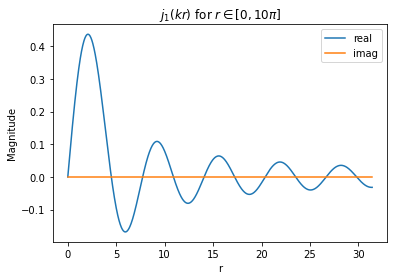
\includegraphics[width=0.6\textwidth]{bessel_zeros.png}
    \caption{Zeros of the first order spherical Bessel function for $k = 1$.}
    \label{fig:bessel_zeros}
\end{figure}


Similarly for interior Neumann problems the same effect can be observed where we instead consider the zeros of the first derivative of the spherical Bessel function. 

This can be shown for \textit{any bounded domain}, using variational methods or Hilbert-Schmidt theory of symmetric integral operators \cite{coltonkress2013}. The set of these numbers are countably infinite. $\mathcal{D}(\Omega)$  are called the set of interior Dirichlet eigenvalues, and $\mathcal{N}(\Omega)$ are called the set of interior Neumann eigenvalues.

In general, for a real $k$ we do not have guaranteed uniquess for interior problems. This is a serious issue, and does cause problems as we formulate our boundary integral equations.

\subsubsection{Boundary Integral Equations}

As we did for Laplace, we can again formulate boundary integral equations based on the representation of our solution as as a double-layer potential.

\begin{flalign}
    u(x) = \int_{\partial \Omega} \frac{\partial \Phi(x, y)}{\partial n(y)}\psi(y) ds(y), \> \> x \in \mathbb{R}^3 \setminus \partial \Omega
\end{flalign}

with a continuous density $\psi$ that solves the boundary integral equation derived from the interior Dirichlet problem,

\begin{flalign}
    &\psi(x) - 2 \int_{\partial D} \frac{\partial \Phi(x, y)}{\partial n (y)}\psi(y) ds(y) = -2f(x), \> \> x \in \partial \Omega \\
    &\psi - K \psi = -2 f
\end{flalign}

For the interior Neumann problem, we wisely (as will be apparent) start of by representing our solution as a single-layer potential instead,

\begin{flalign}
    u(x) = \int_{\partial \Omega} \Phi(x, y) \psi(y) ds(y), \> \> x \in \mathbb{R}^3 \setminus \partial \Omega
\end{flalign}

Taking the normal derivative at the targets,

\begin{flalign}
    \frac{\partial u(x)}{\partial n (x)} = \int_{\partial \Omega} \frac{\partial \Phi(x, y)}{\partial n (x)} \psi(y) ds(y)
\end{flalign}

and applying the jump relation to get our integral equation in terms of Neumann data and the single layer acoustic density,

\begin{flalign}
    &\int_{\partial \Omega} \frac{\partial \Phi(x, y)}{\partial n (x)} \psi(y) ds(y) + \frac{1}{2}\phi(x) = g(x), \> \> x \in \partial \Omega \\
    &\phi + K'\phi = 2g
\end{flalign}

Repeating this trick for the exterior Neumann and Dirichlet problems, we get a set of integral equations. For the interior and exterior Dirichlet problems,

\begin{flalign}
    \psi - K\psi = -2f \\ 
    \psi + K \psi = 2f
\end{flalign}

and for the interior and exterior Neumann problems,

\begin{flalign}
    \phi + K'\phi = 2g \\
    \phi - K'\phi = -2g
\end{flalign}

We observe the duality between the interior Dirichlet / exterior Neumann problem, and vice versa. This basically means, going back to our preliminary theory, that the nullspace of $(I+K)$ corresponds to the solution space of the homogenous interior Neumann problem. They prove this on p81 of \cite{coltonkress2013}. Ok, why does this matter? Well, it matters because our solution space for the homogeneous interior Neumann problem is degenerate at the values of Neumann eigenvalues, so we lose uniqueness for the exterior Dirichlet problem by our choice of formulation! This is annoying, as we know that the exterior Dirichlet problem is uniquely determined, due to Rellich's famous lemma p78 \cite{coltonkress2013}. This is true also for the adjoint problem, where the exterior Neumann problem fails to be uniquely resolvable in our formulation at wave numbers corresponding to Dirichlet eigenvalues.

\subsubsection{Boundary Integral Equations of the First Kind}

Let's now try to formulate first kind equations, we'll see that this approach is still fraught with difficulties.

For the Dirichlet problem, we get a first-kind equation by representing the solution as a single-layer potential,

\begin{flalign}
    u(x) = \int_{\Omega} \Phi(x, y)\phi(y) ds(y), \> \> x \in \mathbb{R}^3 \setminus \partial D
\end{flalign}

This solves the interior and exterior Dirichlet problem, as long as the density satisfies the boundary integral equation,

\begin{flalign}
    \int_{\partial \Omega} \Phi(x, y) \phi(y) ds(y), \> \> x \in \partial \Omega
\end{flalign}

or 

\begin{flalign}
    \mathcal{S}\phi = f
\end{flalign}

This is a first-kind equation, and falls out of the realm of our well-developed Riesz-Fredholm theory. We can still try and solve it with some trickery to force it back into our theoretical framework. From the definition of the single-layer jump relation,

\begin{flalign}
    \phi := \frac{\partial u_-}{\partial n} -  \frac{\partial u_+}{\partial n}, \> \> \text{on } \partial \Omega
\end{flalign}

Consider a representation in terms of a double layer potential to solve the interior Dirichlet problem,

\begin{flalign}
    \psi = -2(I-K)^{-1}f
\end{flalign}

similarly, for the exterior Dirichlet problem,

\begin{flalign}
    \psi = 2(I+K)^{-1}f
\end{flalign}

Now, let us try and solve the Neumann problems using our hypyersingular operator and a double layer potential,

\begin{flalign}
    u(x) = \int_{\partial \Omega} \frac{\partial \Phi(x, y)}{\partial n (y)} \psi(y) ds(y), \> \> x \in \mathbb{R} \setminus \partial D
\end{flalign}

we get the boundary integral equation,

\begin{flalign}
    \frac{\partial}{\partial n (x)} \int_{\partial \Omega} \frac{\partial \Phi(x, y)}{\partial n (y)} \psi(y) ds(y) = g(x), \> \> x \in  \partial D
\end{flalign}

which is `hypersingular', we can write it in operator form as,

\begin{flalign}
    T \psi = 2g = 2 \frac{\partial u}{\partial n}
\end{flalign}

Therefore, we can now see that,

\begin{flalign}
    u &:= T\psi_- - T\psi_+ \\
    u &= -2 T((I-K)^{-1} - (I+K)^{-1})f\\
    u &= -2T(I-K)^{-1}(I+K)^{-1}f
\end{flalign}

where the last line follows by identity. So we identify the solution operator with,

\begin{flalign}
    S^{-1} = -2T(I-K)^{-1}(I+K)^{-1}
\end{flalign}

This allows us to solve the first-kind equation, which we've craftily embedded into our second-kind framework. $T$ is not bounded, so the system is very ill-conditioned and subject to large perturbations with small perturbations in the input.

\subsection{Vector Helmholtz (Maxwell)}

\printbibliography[heading=bibintoc]

\end{document}


